\documentclass[tikz, border=12]{standalone}
\usepackage{stix}
\usepackage{tikz, tkz-euclide, pgfmath, pstricks}
\usetikzlibrary{intersections, decorations.markings, angles,
quotes, calc, arrows, arrows.meta}
\usetkzobj{all}
%
\definecolor{blue}{RGB}{0,51,255}
\definecolor{green}{RGB}{0,153,0}
\definecolor{blue1}{RGB}{174,214,241}
\colorlet{dcolor}{blue}
%
\begin{document}
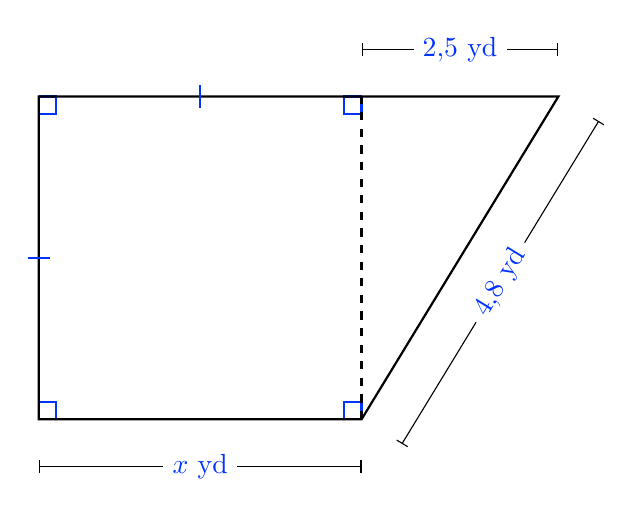
\begin{tikzpicture}
\pgfgettransformentries{\mya}{\myb}{\myc}{\myd}{\mys}{\myt}
\pgfmathsetmacro{\preserve}{1/\mya}
\begin{scope}[>={Stealth[scale=1.2]} , thick,rotate=0 ] 
\def \s{4.1}
\def \ad{2.5+4.1}
\coordinate (b) at (0,0); 
\coordinate (c) at (\s,0); 
\coordinate (x) at (\s,\s); 
\coordinate (a) at (0,\s); 
\coordinate (d) at (\ad,\s); 
\tkzMarkRightAngle[size=0.22*\preserve, color=blue,thick](b,a,x);
\tkzMarkRightAngle[size=0.22*\preserve, color=blue,thick](c,b,a);
\tkzMarkRightAngle[size=0.22*\preserve, color=blue,thick](x,c,b);
\tkzMarkRightAngle[size=0.22*\preserve, color=blue,thick](a,x,c);
\draw (a)--(b)--(c)--(d)--cycle;
\draw [dashed] (c)--(x);
%
\draw[|-|,thin] ($(c)!-6mm*\preserve!90:(d)$)--node[color=blue,fill=white,sloped] {$4{,}8\ \textrm{yd}$} ($(d)!-6mm*\preserve!-90:(c)$);
\draw[|-|,thin] ($(d)!-6mm*\preserve!90:(x)$)--node[color=blue,fill=white,sloped] {$2{,}5\ \textrm{yd}$} ($(x)!-6mm*\preserve!-90:(d)$);
\draw[|-|,thin] ($(b)!-6mm*\preserve!90:(c)$)--node[color=blue,fill=white,sloped] {$x\ \textrm{yd}$} ($(c)!-6mm*\preserve!-90:(b)$);
%
\tkzMarkSegment[color=blue, pos = 0.5,mark=|](a,x)
\tkzMarkSegment[color=blue, pos = 0.5,mark=|](a, b)



\end{scope}
\end{tikzpicture}
\end{document}
